\section{The Disaster Scenario}\label{sec:scenario}
\noindent To develop a scenario for the evaluation of agent-based planning support, we held a number of consultations with emergency response organisations such as Rescue Global\footnote{\url{http://www.rescueglobal.org.}} and Hampshire County Council.\footnote{\url{http://www3.hants.gov.uk/emergencyplanning.htm.}} Specifically,  these discussions informed the design of decision-making challenges  (e.g., hazard avoidance, path planning, team coordination) that mimic those that pervade real-world disaster response planning and execution while making reasonable assumptions about the environment and the participants.\footnote{As access to emergency responders is either limited or costly for field trials, it was considered reasonable to hire volunteers that were taught to use the tools we gave them. The design of a fully-fledged training tool for disaster responder would be beyond the scope of this paper.}  

In more detail, we consider a disaster scenario in which a satellite, powered by radioactive fuel,  has crashed in a sub-urban area.\footnote{Given the invisibility of radiation, it is possible to create a believable and challenging environment for the responders to solve in our mixed-reality game (see Section \ref{sec:atomicorchid}).} Debris is strewn around a large area, damaging buildings and causing accidents and injuring civilians. Moreover, radioactive particles discharged from the debris are gradually spreading over the area, threatening to contaminate food reserves and people. As the movement of this radioactive cloud is dependent on wind speed and direction, radiation levels may change drastically across the disaster space over time (see Appendix \ref{sec:radiation} for more details of the model we use). Hence, emergency services (including medics, soldiers, transporters, and fire-fighters) are deployed to  evacuate the casualties and key assets (e.g., food reserves, medication, fuel), each requiring different teams of FRs, before they are engulfed by the radioactive cloud.  In what follows, we first model this scenario formally. Second, we describe the use of a planning agent at headquarters to help coordinate the team. Third, we formalise  the optimisation problem faced by the planning agent in trying to coordinate the team of FRs on the ground (i.e., including fire-fighters, medics, and soldiers) with the objective o save as many lives and assets as possible while minimising the risk of being exposed to harmful radiation.  

%We then propose an algorithm to solve this optimisation problem (in Section \ref{sec:algo}). In Section \ref{sec:atomicorchid}, we demonstrate how this algorithm can be used by a software agent (in our mixed-reality game) in a mixed-initiative process to coordinate first responders. 

\subsection{Formal Model}\label{sec:model}
\noindent Let $G$ denote a grid overlaid on top of the disaster space, and assume the satellite debris, casualties, assets, and actors are located at various coordinates $(x,y) \in G$ in this grid. The radioactive cloud induces a radioactivity level  $l \in [0,100]$ at every point it covers (100 corresponds to maximum radiation and 0 to no radiation). While the exact radiation levels can be measured by responders on the ground (at a given location) using their geiger counter, we assume that additional information is available  from existing sensors  in the area.\footnote{This assumption is not central to our problem and only serves to inform the decision making of the agent as we see later. It is also possible to obtain similar information about radiation levels by fusing the responders' geiger counter readings, but this is beyond the scope of the paper.} However, this information is uncertain due to the poor positioning of the sensors and the variations in wind speed and direction (we show how this uncertainty is captured in the next section). A number of safe zones $G' \subseteq G$ are defined where the responders can drop off assets and casualties (i.e., \emph{targets} to be rescued). Let the set of FRs be denoted as $I = \{p_1, \cdots p_i \cdots, p_n\}$, where $|I| = n$ and the set of  targets to be rescued (i.e., rescue tasks) be denoted as  $T = \{t_1,\cdots, t_j, \cdots, t_m\}$, where $|T| = m$. A rescue task is performed by picking the target up, carrying it to a safe zone, and dropping it off.  As FRs perform rescue tasks, they may become tired, get injured, or receive radiation doses that may, at worst, be life threatening. Hence, we assign each responder  a health level $h_i\in [0,100]$ that decreases based on its radiation dose ($h_i$ is decreased by $0.02 \times l$ per second given a radiation level $l$) and assume that its decision to pick up and carry the target allocated to it is liable to some uncertainty (e.g., they may not want to pick a target because it is too far away or it is unclear how long it is going to take them to  carry it back  to a safe zone).  Moreover, let $\Theta$ denote the types of responders (e.g., fire brigade, soldier, transporter, or medic)  and assume a responder's type determines the capabilities  she has and therefore the tasks  she can perform. We denote as $\theta_i \in \Theta$ the type of responder $p_i$. In turn, to complete a given task $t_j$,  a set of responders $C \subseteq I$ with specific types $\Theta_{t_j} \subseteq \Theta$ is required to pick up $t_j$. Thus, a task can only be completed by a team of responders $C_j$ if $\{\theta_i | p_i \in C_j\} \subseteq \Theta_{t_j}$. Given the distribution of responders across the physical space, different sub-teams will perform to different levels (as they have to travel different distances) and this poses a challenge for the commander and to find the best teams needed to perform the tasks.
%\begin{figure}[htbp]
%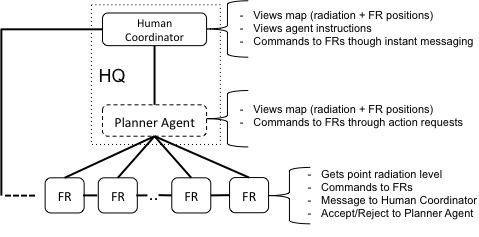
\includegraphics[width=\columnwidth]{scenario.jpg}\vspace{-5mm}
%
%\label{fig:scenario}
%\caption{The interactions between different actors in the disaster scenario. Lines represent communication links. Planner agent and coordinator sit in the headquarters (HQ). First responders (FRs) can communicate with all actors directly.}\end{figure}
\subsection{Human-Agent Collaboration}
\noindent In line with practice in many countries, we assume that the FRs are coordinated from a headquarters (HQ) headed by a human coordinator $H$. In our case, $H$ is assisted by an agent-based planning agent $PA$ (more details in Section \ref{sec:algo}), that can receive input from, and direct, the FRs.   Both  $H$ and $PA$  can communicate their  instructions (task plans to pick up targets) directly to the responders using an instant messaging system (or walkie talkie).  While these instructions may be in natural language for $H$, $PA$ instructs them with simple requests such as ``Pick up target X at position Y with team-mates Z'' messages. In turn, the responders may not want to do some tasks (e.g., if they are too tired, prefer to work with specific  peers, or are prioritise some tasks over others) and may therefore simply accept or reject the received instruction from $PA$ or $H$.\footnote{While some agencies may be trained to obey orders (e.g., military or fire-fighting), others (e.g., transport providers or medics) are not  always trained to do so \cite{harvard2010disaster}.} However, $H$ can query the responders' decisions and request  more information about their status (e.g., fatigue or health) and goals (e.g., meeting with team-mate at position X or going for task Y). Instead, if a task is rejected by the responders, $PA$ records this as a constraint on its task allocation procedure (see details in Section \ref{sec:adaptive}) and returns a new plan. Thus on the one hand, richer interactions are possible between $H$ and the first responders than between them and $PA$. On the other hand, $PA$ runs an sophisticated task allocation algorithm that can compute an efficient allocation, possibly better than the one computable by $H$ (particularly when many responders need to be managed). Note that, in contrast to previous work that suggested \emph{transfer-of-control} regimes \cite{scerri:etal:2005}, our approach to handling requests from FRs to change the agent-based plan, does not constrain transfers of control to target specific decision points in the operation of the system. Rather, our interaction mechanisms are designed (see Section \ref{sec:atomicorchid}) to be more flexible to allow human control at any point (and our results  in Section \ref{sec:evaluation} validate this approach), along with human supervision (to implement possible corrective actions) by $H$.

\subsection{The Optimisation Problem}
\label{sec:model}
\noindent Previous agent-based models for team coordination in disaster response typically assume deterministic task executions and environments \cite{ramchurn:etal:2010,Scerri2005}. However, in order to evaluate agent-guided coordination in a real-world environment, it is important to consider uncertainties due to player behaviours and the environment (as discussed in the previous section). Given this, we propose a new representation for the task allocation problem in disaster response that does take into account such uncertainties. More specifically, we represent this problem using an MMDP that captures the uncertainties of the radioactive cloud and the responders' behaviours. We model the spreading of the radioactive cloud as a random process over the disaster space and allow the actions requested from the responders to  fail (because they decline to go to a  task) or incur delays (because they are too slow) during the rescue process. Thus in the MMDP model, we represent  task executions as stochastic processes of state transitions, while the uncertainties of the radioactive cloud and the responders' behaviours can be easily captured with transition probabilities.  More formally, the MMDP is
represented by tuple $\mathcal{M} = \langle I, S, \{A_i\}, P, R
\rangle$, where $I$ is the set of actors as defined in the previous
section,  $S$ is the state space, $A_i$ is a set of responder
$p_i$'s actions, $P$ is the transition function, and $R$ is the
reward function. We elaborate on each of these below.

In more detail, $S= S^G_r \times S_{p_1} \times \cdots \times
S_{p_n} \times S_{t_1} \times \cdots \times S_{t_m}$ where $S^G_r =
\{l_{(x,y)}| (x, y) \in G\}$ is the state variable of the
radioactive cloud that specifies the radioactive level
$l_{(x,y)}\in[0, 100]$ at every point $(x, y)\in G$. $S_{p_i} =
\langle h_i, (x_i, y_i), t_j \rangle$ is the state variable for
each responder $p_i$ that specifies her health level
$h_i\in[0, 100]$, her present position $(x_i, y_i)$, and the task
$t_j$ she is carrying out. $S_{t_j} = \langle {\tt st_j}, (x_j, y_j)
\rangle$ is then the state variable for task $t_j$ to specify its
status ${\tt st_j}$ (i.e., the target is picked up, dropped off, or idle) and position $(x_j, y_j)$. 

The three types of actions  (in set $A_i$) a responder can take
are: (i) {\em stay} in the current location $(x_i, y_i)$, (ii) {\em
move} to the 8 neighbouring locations, or (iii) {\em complete} a
task located at $(x_i, y_i)$. A joint action $\vec{a}=\langle a_1,
\cdots, a_n \rangle$ is a set of actions where $a_i\in A_i$, one
for each responder (a responder may just \emph{stay} at its current
position if it has no targets to rescue). The transition function
$P$ is defined in more detail as: $P= P_r \times P_{p_1} \times
\cdots \times P_{p_n} \times P_{t_1} \times \cdots \times P_{t_m}$
where:
\begin{itemize}
    \itemsep=-2pt
    \item $P_r(s'_r|s_r)$ is the probability the radioactive
        cloud spreads from state $s_r\in S^G_r$ to $s'_r\in
        S^G_r$. It captures the uncertainty of the  radiation
        levels in the environment due to  noisy sensor readings
        and the variations in wind speed and direction.
    \item $P_{p_i}(s'_{p_i}|s, a_i)$ is the probability
        responder $p_i$ transitions to a new state $s'_{p_i}\in
        S_{p_i}$ when executing action $a_i$. For example, when
        a responder is asked to go to a new location,  she
        may not end up there because  she is tired,
        gets injured, or receives radiation doses that are life
        threatening.
    \item $P_{t_j}(s'_{t_j}|s, \vec{a})$ is the probability
        of task $t_j$ being completed. A task $t_j$ can only be completed by a
        team of responders with the required types ($\Theta_{t_j}$) located at the
        same position as $t_j$.
\end{itemize}

Now,  if  $t_j$ is completed (i.e., in ${\tt st_j}\in S_{t_j}$, the
status ${\tt st_j}$ is marked as ``dropped off'' and its position $(x_j,
y_j)$ is within a safe zone), the team will be rewarded using
function $R$. The team is penalised if a responder $p_i$ gets
injured or receives a high dose of radiation (i.e., in $s_{p_i}$,
the health level $h_i$ is 0). Moreover, we attribute a cost to each
of the responders' actions since  each  action requires them to
exert some effort (e.g., running or carrying objects).


Give the above definitions, a policy for the MMDP is a mapping from
states to joint actions, $\pi: S \rightarrow \vec{A}$ so that the
responders know which actions to take given the current state of
the problem. The quality of a policy $\pi$ is  measured by
its expected value $V^\pi$, which can be computed recursively by
the Bellman equation:
\begin{equation}
  V^\pi(s^\tau) = R(s^\tau, \pi(s^\tau)) + \!\!\!\sum_{s^{\tau+1}\in S}\!\!\!
  P(s^{\tau+1}|s^\tau, \pi(s^t)) V^\pi(s^{\tau+1})
\end{equation}
where $\tau$ denotes the current time point and $\pi(s^\tau)$ is a joint action given $s^\tau$. The goal of solving
the MMDP is to find an optimal policy $\pi^*$ that maximises the
expected value with the initial state $s^0$, $\pi^* =
\arg\max_{\pi} V^\pi(s^0)$.

At each decision step, we assume the planning agent can fully
observe the state of the environment $s$ by collecting sensor
readings of the radioactive cloud and GPS locations of the
responders. Given a policy $\pi$ of the MMDP, a joint action
$\vec{a}=\pi(s)$ can be selected and broadcast to the responders
(as mentioned earlier).

